
\documentclass[10pt]{article}
\usepackage[utf8]{inputenc}
\usepackage[T1]{fontenc}
\usepackage{lmodern}
\usepackage[margin=0.72in]{geometry}
\usepackage{amsmath,amssymb,amsthm}
\usepackage{booktabs,longtable,array,multirow,tabularx}
\usepackage{graphicx}
\usepackage{float}
\usepackage{xcolor}
\usepackage{hyperref}
\usepackage{enumitem}
\usepackage{caption}
\usepackage{microtype}
\usepackage{mathtools}
\hypersetup{colorlinks=true,linkcolor=blue,citecolor=blue,urlcolor=blue}
\setlength{\parskip}{0.48em}
\setlength{\parindent}{0pt}
\setlist[itemize]{leftmargin=1.2em,itemsep=0.15em,topsep=0.25em}
\setlist[enumerate]{leftmargin=1.5em,itemsep=0.15em,topsep=0.25em}
\emergencystretch=3em
\sloppy
\makeatletter
\renewcommand*\l@section{\@dottedtocline{1}{1.5em}{7.2em}}
\makeatother
\newcommand{\SY}{\mathfrak{S}_Y}
\newcommand{\CHLone}{\mathrm{CHL1}}
\newcommand{\CHLtwo}{\mathrm{CHL2}}
\newcommand{\Epath}{E_Y^{\mathrm{path}}}
\newcommand{\Omegapath}{\Omega_Y^{\mathrm{path}}}
\newcommand{\oneadm}{\mathbf{1}_{\mathrm{adm}}}
\newcommand{\loglik}{\ell}
\title{CHL2: A Conditional Hardy--Littlewood Markov Kernel for Consecutive Prime Gaps}
\author{Jose Antonio Cano Gregorio}
\date{Whitepaper v1.3 --- Final Release Candidate (Pre-submission Review)}
\begin{document}
\maketitle
\begin{abstract}
\noindent\textbf{Whitepaper v1.3 --- Final Release Candidate (Pre-submission Review).}\par
This paper introduces CHL2, a finite conditional Markov kernel for consecutive prime gaps obtained by factorizing the Hardy--Littlewood singular-series heuristic into a transition law.  If $g_1=p_{n+1}-p_n$ is the previous gap and $g_2=p_{n+2}-p_{n+1}$ is the next candidate gap, the CHL1 factor is the conditional singular-series ratio
\[
R_Y(g_2\mid g_1)=\frac{\SY(\{0,g_1,g_1+g_2\})}{\SY(\{0,g_1\})}.
\]
CHL2 adds a first-order Poisson no-interior-prime survival factor derived from conditional four-point singular-series ratios,
\[
\Epath(g_1,g_2;x)=\exp\!\left[-\sum_{\substack{2\le u\le g_2-2\\u\ \mathrm{even}}}\frac{1}{\log x}\frac{\SY(\{0,g_1,g_1+u,g_1+g_2\})}{\SY(\{0,g_1,g_1+g_2\})}\right].
\]
Thus the model weights not only the three endpoint positions but also the absence of a prime in the future interval, which is the missing consecutiveness condition in a triple-constellation model.

The empirical DS1 audit covers ten sequential blocks near $10^{11}$ and $78{,}934{,}825$ observed transitions. At $Y=47$ (truncation horizon), CHL2 path-exclusion is the best conditional log-likelihood model in every evaluated stratum and improves the CHL1 ratio-only kernel in all filters. A cutoff sweep over $Y\in\{31,47,61,73\}$ preserves the sign of the gain in every stratum and against classical zero-memory baselines, including Cramer--Granville variants. An absolute prime-residue Oliver--Soundararajan diagnostic gives partial validation: strong agreement in modulus $7$, moderate agreement in modulus $5$, and a documented wrong-sign limitation in modulus $3$.

The paper does not claim a proof of the Riemann Hypothesis, Goldbach's conjecture, the twin-prime conjecture, or any new asymptotic theorem on prime gaps. The claim is narrower: CHL2 is a finite, parameter-free conditional kernel, once $Y$ and the local scale are fixed, derived from classical singular-series structure and a first-order no-interior survival correction. A final forward-looking section proposes a heuristic variational bridge from conditional kernels to adaptive sieve weights; it is explicitly not presented as a proven result.
\end{abstract}
\tableofcontents
\listoffigures
\newpage
\section{Introduction}
Classical sieve theory and the Hardy--Littlewood heuristic assign weights to admissible configurations and use those weights to estimate densities, moments, or existence statements. CHL2 asks a related but different question: after a gap $g_1$ has just occurred, how should the next candidate gap $g_2$ be weighted as a conditional transition?
\[
\boxed{\text{Hardy--Littlewood gives static constellation weights; CHL2 studies their conditional Markov factorization.}}
\]
This phrasing is deliberately conservative. CHL2 does not replace the singular series; it uses it. Nor does CHL2 produce a new analytic sieve theorem. It produces a finite conditional kernel that can be audited against observed consecutive-gap transitions and compared against zero-memory baselines. The project was originally motivated by empirical path-geometry features, but the present kernel removes those fitted geometric coefficients from the core.\footnote{The previous fitted geometric features are retained only as historical context and possible residual diagnostics. The core model analyzed here uses singular-series ratios and no-interior survival factors, not Shape/Balance/Tail coefficients.}
\subsection{Relation to modern prime-gap work}
Modern work on prime gaps uses residue classes, admissible tuples, multidimensional sieve weights, probabilistic selection, and covering arguments. Maynard's large-gap work and the Ford--Green--Konyagin--Maynard--Tao long-gap framework use these tools to prove asymptotic existence results for long prime gaps \cite{maynard-large,ford2016}. Maynard--Tao/GPY/Zhang-type methods address bounded gaps and dense admissible tuples through optimized sieve weights \cite{gpy,maynard-small,zhang}. These works are analytic theorems about limiting behavior. CHL2 is not such a theorem; it is a finite conditional model tested on observed consecutive gaps.

The overlap is structural, not competitive. Both settings use admissibility and local congruence factors. The difference is the object being optimized or measured. Classical sieve arguments usually optimize sums over configurations. CHL2 defines a transition law $P(g_2\mid g_1,x)$ for the next gap after a known previous gap. This is why the output is described as a Markov kernel rather than as a new singular-series conjecture.
\subsection{Claims and non-claims}
The evidence in this paper supports the following limited claims.
\begin{enumerate}
\item The conditional singular-series ratio $\SY(H_3)/\SY(H_2)$ is an effective Markov factor for consecutive-gap transitions.
\item The no-interior-prime correction $\Epath$ improves the ratio-only kernel in the DS1 audit without adding empirical coefficients.
\item The improvement is stable in sign across $Y\in\{31,47,61,73\}$.
\item The local memory $g_1\mapsto g_2$ is operationally irreducible relative to zero-memory baselines in the reported likelihood metrics.
\item The absolute prime-residue test provides partial, not complete, Oliver--Soundararajan-style validation.
\end{enumerate}
We do not claim that CHL2 proves any open conjecture. We do not claim that CHL2 improves theorems of Maynard, Tao, Selberg, Granville, or Hardy--Littlewood. We do not claim that the first-order Poisson exclusion term is the final analytic expression for consecutiveness. It is the strongest parameter-free conditional model tested so far in this finite audit.
\section{Definitions and finite truncation}
Let $p_1<p_2<p_3<\cdots$ be the increasing sequence of primes. Consecutive gaps are $g_n=p_{n+1}-p_n$. For two consecutive gaps we write $g_1=p_{n+1}-p_n$ and $g_2=p_{n+2}-p_{n+1}$. The pair $(g_1,g_2)$ encodes a length-two path in the prime sequence.

Fix a finite truncation horizon $Y$ and define the truncated singular series of a finite set $H\subset\mathbb Z$ by
\[
\SY(H)=\prod_{q\le Y}\frac{1-\nu_q(H)/q}{(1-1/q)^{|H|}},
\]
where $\nu_q(H)$ is the number of distinct residue classes occupied by $H$ modulo the prime $q$. A set $H$ is admissible at horizon $Y$ if
\[
\nu_q(H)<q\qquad\text{for every prime }q\le Y.
\]
Equivalently, if $\nu_q(H)=q$ for some $q\le Y$, the local factor vanishes, the tuple is inadmissible at horizon $Y$, and the kernel assigns it a hard zero.

For $p_n>2$, candidate prime gaps are even. All normalizing sums in this paper are therefore taken over even candidate gaps $g_2\ge2$. This convention is part of the model support, not a fitted assumption. All subsequent kernels inherit this admissibility support and even-gap restriction.

The endpoint sets used in CHL1 are $H_2(g_1)=\{0,g_1\}$ and $H_3(g_1,g_2)=\{0,g_1,g_1+g_2\}$. The four-point set used for interior exclusion is $H_4(u;g_1,g_2)=\{0,g_1,g_1+u,g_1+g_2\}$, with $2\le u\le g_2-2$ and $u$ even.

The horizon $Y$ should not be confused with a classical sieve level. It is an auditable truncation horizon for a finite empirical kernel. The choice of $Y=47$ acts as an auditable truncation horizon for empirical validation and stability sweeps; we do not assert asymptotic convergence, only that the Markov kernel improvement is stable across this evaluated range.
\section{CHL1: conditionalizing Hardy--Littlewood}
The static Hardy--Littlewood triple weight $\SY(H_3)$ gives the arithmetic weight of the three endpoint positions as a constellation. It does not by itself express a transition law after the pair $H_2(g_1)$ has already been observed.
\[
R_Y(g_2\mid g_1)=\frac{\SY(H_3(g_1,g_2))}{\SY(H_2(g_1))}.
\]
Expanding logarithmically,
\[
\log R_Y(g_2\mid g_1)=\sum_{q\le Y}\left[\log\left(1-\frac{\nu_q(H_3)}{q}\right)-\log\left(1-\frac{\nu_q(H_2)}{q}\right)-\log\left(1-\frac{1}{q}\right)\right].
\]
This is the first point where memory appears without being postulated. The previous gap $g_1$ changes the residue pattern of $H_3$, and therefore changes the local factors in the ratio.

A normalized CHL1 kernel is
\[
P_Y^{\CHLone}(g_2\mid g_1;x)=\frac{\mathbf{1}_{\mathrm{adm},Y}^{(3)}(g_1,g_2)R_Y(g_2\mid g_1)\exp(\eta_Y(x)g_2)}{Z_Y^{\CHLone}(g_1;x)},
\]
where
\[
Z_Y^{\CHLone}(g_1;x)=\sum_{\substack{h\ge 2\\h\ \mathrm{even}}}\mathbf{1}_{\mathrm{adm},Y}^{(3)}(g_1,h)R_Y(h\mid g_1)\exp(\eta_Y(x)h).
\]
The scalar $\eta_Y(x)$ is a Lagrange multiplier used to impose the finite-window mean-gap scale. In the reported implementation, $\eta_Y$ is solved numerically within the evaluated support so that the model mean of $g_2$ matches the empirical/PNT local scale in that block and stratum. On a finite even support, this exponential-family mean is monotone in $\eta_Y$ whenever the support has nonzero variance; hence the anchoring equation has a unique solution and is solved stably by bisection/Newton search. Thus $\eta_Y$ is not a fitted local feature: its value is determined by the PNT/empirical scale anchor within the finite support. While CHL1 captures path-dependent arithmetic weight, it does not enforce strict consecutiveness.
\section{CHL2: adding no-interior-prime exclusion}
CHL1 models the three endpoints as a prime-like constellation. Consecutive gaps require more: there must be no prime in the future interval between the second and third endpoints.
\subsection{Derivation of the path-sensitive interior intensity}
Condition on $H_3=\{0,g_1,g_1+g_2\}$. For an interior candidate position $g_1+u$, with $2\le u\le g_2-2$ and $u$ even, define $H_4(u)=\{0,g_1,g_1+u,g_1+g_2\}$. Under the same truncated Hardy--Littlewood heuristic, the relative intensity that the interior position is also prime-like, conditional on the endpoint triple, is
\[
I_Y(u\mid g_1,g_2;x)=\frac{1}{\log x}\frac{\SY(H_4(u))}{\SY(H_3)}.
\]
For numerical stability in DS1, we approximate $\log(p_n+g_1+u)$ by a local constant $\log x$ with $x\approx10^{11}$; the maximum relative variation across the evaluated DS1 window is below $2\%$. A pointwise version using $\log(p_n+g_1+u)$ is a trivial refinement for cross-scale audits, but it was not needed for the present finite-window validation.

Assuming a first-order Poisson survival approximation, the expected number of interior prime-like points is
\[
\Omegapath(g_1,g_2;x)=\sum_{\substack{2\le u\le g_2-2\\u\ \mathrm{even}}} I_Y(u\mid g_1,g_2;x),
\]
and $\Epath(g_1,g_2;x)=\exp(-\Omegapath(g_1,g_2;x))$. Note that $\Epath\in(0,1]$ acts as a soft survival penalty, complementing the hard admissibility mask. The word ``Poisson'' is used narrowly: this is a first-order survival approximation, not an asymptotic theorem. Second-order inclusion--exclusion among multiple interior points remains a future refinement. In this paper its adequacy is tested indirectly through the CHL2-vs-CHL1 likelihood gain and the path-vs-gap comparison; a direct cluster-expansion validation is left to future work.
\subsection{The CHL2 path-exclusion kernel}
The core model audited in this paper is
\[
\boxed{P_Y^{\CHLtwo}(g_2\mid g_1;x)=\frac{\mathbf{1}_{\mathrm{adm},Y}^{(3)}(g_1,g_2)R_Y(g_2\mid g_1)\Epath(g_1,g_2;x)\exp(\eta_Y(x)g_2)}{Z_Y^{\CHLtwo}(g_1;x)}}.
\]
The normalization is explicitly over even candidate gaps:
\[
Z_Y^{\CHLtwo}(g_1;x)=\sum_{\substack{h\ge 2\\h\ \mathrm{even}}}\mathbf{1}_{\mathrm{adm},Y}^{(3)}(g_1,h)R_Y(h\mid g_1)\Epath(g_1,h;x)\exp(\eta_Y(x)h).
\]
Equivalently, the log-score before normalization is $\log R_Y(g_2\mid g_1)-\Omegapath(g_1,g_2;x)+\eta_Y(x)g_2$.

A faster diagnostic version uses only future-gap endpoints,
\[
\Omega_Y^{\mathrm{gap}}(g_2;x)=\sum_{\substack{2\le u\le g_2-2\\u\ \mathrm{even}}}\frac{1}{\log x}\frac{\SY(\{0,u,g_2\})}{\SY(\{0,g_2\})}.
\]
This is useful as a baseline, but it does not condition on the full path.
\section{Experimental design}
\subsection{Baselines}
The audit compares CHL2 against: CHL1 ratio-only; noPhi conditional support; HL2 order-zero; HL2 gap-exclusion order-zero; Cramer order-zero; Cramer--Granville order-zero; and Cramer--Granville with gap-exclusion. The important separation is between order-zero and order-one models. Order-zero models may know the candidate gap and finite admissible support, but they do not condition on $g_1$. CHL2 is order-one.
\subsection{Data and strata}
The empirical window consists of ten sequential DS1 blocks near $10^{11}$ with $78{,}934{,}825$ observed transitions. The blocks are chronological windows, not randomly shuffled samples, which is essential for a Markov transition audit. The main run uses $Y=47$ as the truncation horizon. The cutoff-sensitivity run evaluates $Y\in\{31,47,61,73\}$. The filters are defined by $m=\max(g_1,g_2)$: \texttt{ALL}, \texttt{LOW\_ONLY\_LE58}, \texttt{MID\_59\_120}, \texttt{MID\_121\_240}, \texttt{MID\_121\_400}, \texttt{NO\_58}, \texttt{NO\_120}, and \texttt{NO\_240}.
\subsection{Metrics}
The primary metric is conditional log-likelihood per event, $\loglik(M)=N^{-1}\sum_i \log P_M(g_{2,i}\mid g_{1,i},x_i)$. Conditional log-likelihood is the standard information-theoretic metric for transition kernels: it is additive across events and penalizes tail misalignment, unlike distance metrics that may compress sparse regimes. We also report conditional cross-entropy and KL divergence. Pairwise gains are $\Delta\loglik(M,B)=\loglik(M)-\loglik(B)$. A positive value means that model $M$ assigns higher observed conditional likelihood than baseline $B$.
\section{Main results at $Y=47$}
The path-sensitive CHL2 model is the best conditional log-likelihood model in every stratum at $Y=47$ (truncation horizon).
\begin{table}[H]\centering\small
\begin{tabular}{llrrr}
\toprule
Filter & Best model & loglik/event & conditional KL & events \\
\midrule
ALL & CHL2\_path & -3.228309 & 0.000902 & 78,934,825 \\
LOW\_ONLY\_LE58 & CHL2\_path & -2.917648 & 0.000279 & 65,834,862 \\
MID\_59\_120 & CHL2\_path & -3.041260 & 0.001105 & 12,360,379 \\
MID\_121\_240 & CHL2\_path & -3.135146 & 0.037488 & 736,978 \\
MID\_121\_400 & CHL2\_path & -3.146972 & 0.043514 & 739,580 \\
NO\_58 & CHL2\_path & -3.161917 & 0.003541 & 13,099,963 \\
NO\_120 & CHL2\_path & -3.147009 & 0.043545 & 739,584 \\
NO\_240 & CHL2\_path & -3.154615 & 1.636241 & 2,606 \\
\bottomrule
\end{tabular}
\caption{Best-model CHL2 path-exclusion metrics at $Y=47$ (truncation horizon). The sparse \texttt{NO\_240} stratum is reported for completeness but is not used as a central claim.}\label{tab:main-chl2}\end{table}
\subsection{Direct gain over CHL1}
\begin{table}[H]\centering\small
\begin{tabular}{lr}
\toprule
Filter & $\Delta\ell$ CHL2 path vs CHL1 \\
\midrule
ALL & +0.000861 \\
LOW\_ONLY\_LE58 & +0.000569 \\
MID\_59\_120 & +0.000350 \\
MID\_121\_240 & +0.000534 \\
MID\_121\_400 & +0.000544 \\
NO\_58 & +0.000409 \\
NO\_120 & +0.000543 \\
NO\_240 & +0.000917 \\
\bottomrule
\end{tabular}
\caption{Direct test of the no-interior correction. Positive values mean that explicit path-sensitive exclusion improves the conditional singular-series Markov kernel.}\label{tab:chl2-vs-chl1}\end{table}
In the full support, the per-event improvement is approximately $8.61\times10^{-4}$ nats. Gains are additive and cumulative across the window: over $78{,}934{,}825$ events this corresponds to a total log-likelihood improvement of roughly $6.8\times10^4$ nats. The full-support gain is positive in all ten sequential blocks, which is the relevant robustness check for a small per-event effect.
\subsection{Path-sensitive exclusion versus gap-only exclusion}
\begin{table}[H]\centering\small
\begin{tabular}{lr}
\toprule
Filter & $\Delta\ell$ path minus gap-only \\
\midrule
ALL & +0.000249 \\
LOW\_ONLY\_LE58 & +0.000214 \\
MID\_59\_120 & +0.000153 \\
MID\_121\_240 & +0.000272 \\
MID\_121\_400 & +0.000273 \\
NO\_58 & +0.000163 \\
NO\_120 & +0.000273 \\
NO\_240 & +0.000694 \\
\bottomrule
\end{tabular}
\caption{Additional improvement of path-sensitive no-interior exclusion over the gap-only no-interior correction.}\label{tab:path-vs-gap}\end{table}
This matters because it shows that consecutiveness is not reduced to a one-gap tail penalty. The full path $g_1\to g_2$ changes the interior-prime intensity through the four-point ratio $\SY(H_4)/\SY(H_3)$.
\begin{figure}[H]\centering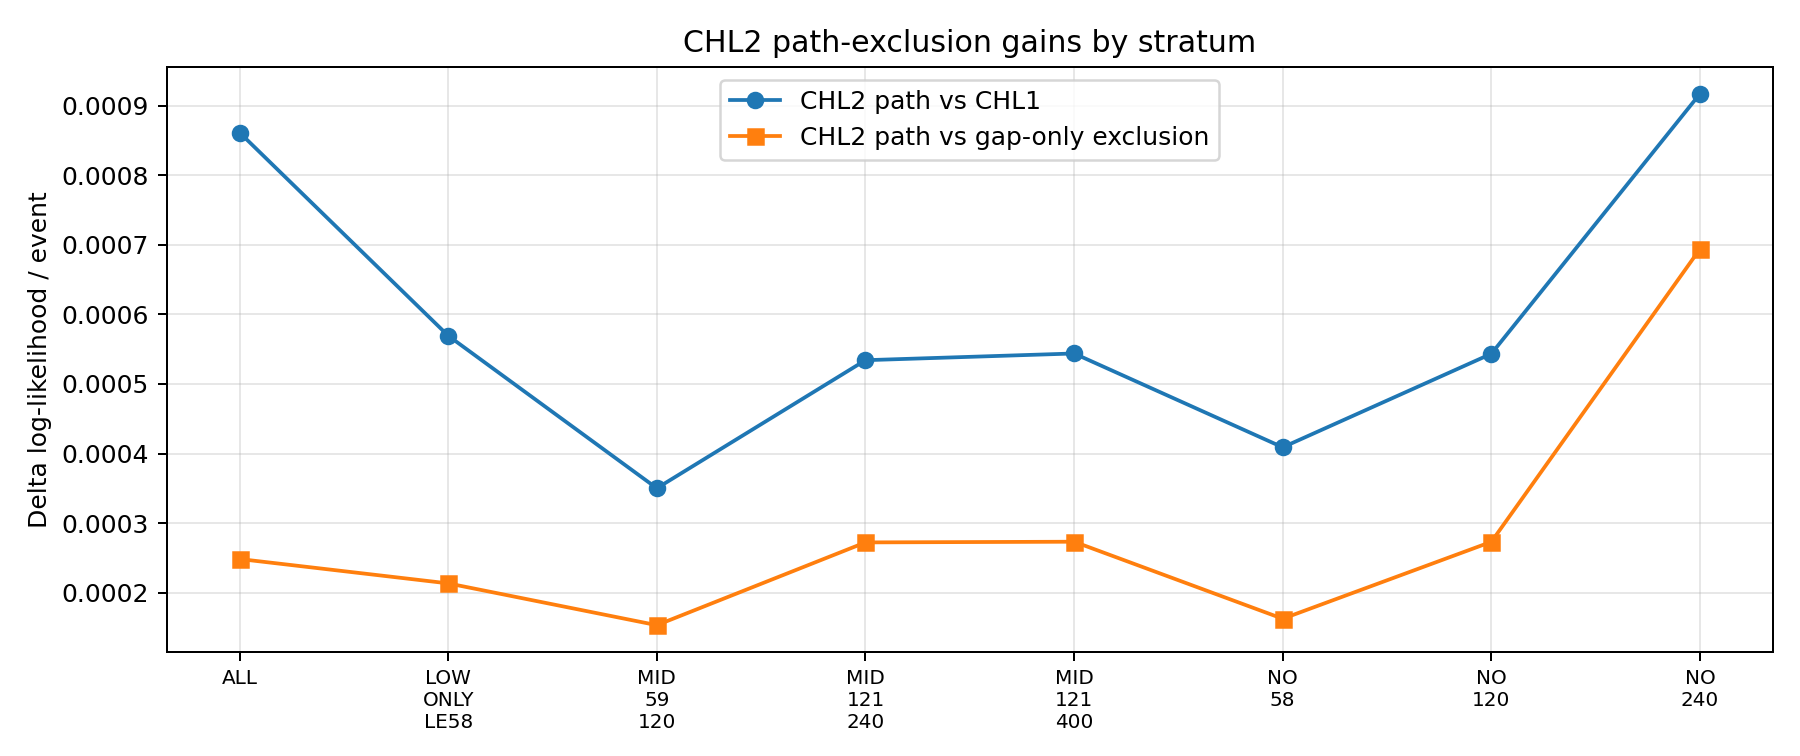
\includegraphics[width=0.94\textwidth]{figures/fig1_chl2_main_gains.png}\caption{CHL2 path-exclusion gains by evaluation stratum.}\end{figure}
\section{Cutoff stability: the $Y$-sweep}
A model that works only at one truncation horizon could be a compression artifact. The cutoff-sensitivity sweep evaluates $Y\in\{31,47,61,73\}$. For each $Y$, the singular-series products and no-interior factors are recomputed. The primary stability criterion is $\min_Y\Delta\loglik_Y(\mathrm{CHL2}_{\mathrm{path}},B)>0$.
\subsection{Stability against CHL1}
\begin{table}[H]\centering\small
\begin{tabular}{lrrr}
\toprule
Filter & min$_Y\Delta\ell$ & mean$_Y\Delta\ell$ & positive $Y$ \\
\midrule
ALL & 0.000840 & 0.000860 & 4/4 \\
LOW\_ONLY\_LE58 & 0.000560 & 0.000567 & 4/4 \\
MID\_59\_120 & 0.000338 & 0.000349 & 4/4 \\
MID\_121\_240 & 0.000534 & 0.000557 & 4/4 \\
MID\_121\_400 & 0.000544 & 0.000566 & 4/4 \\
NO\_58 & 0.000395 & 0.000408 & 4/4 \\
NO\_120 & 0.000543 & 0.000566 & 4/4 \\
NO\_240 & 0.000843 & 0.000905 & 4/4 \\
\bottomrule
\end{tabular}
\caption{Cutoff stability of CHL2 path-exclusion versus CHL1 ratio-only. The sign of the gain is stable over $Y\in\{31,47,61,73\}$.}\label{tab:y-stability}\end{table}
The smallest gain across $Y$ in the full support is $0.000840$ nats/event, still positive. This confirms that the no-interior correction is not an artifact of selecting $Y=47$ alone. Stability here refers to the sign and magnitude of the likelihood improvement, not to convergence of the infinite Hardy--Littlewood product itself.
\begin{figure}[H]\centering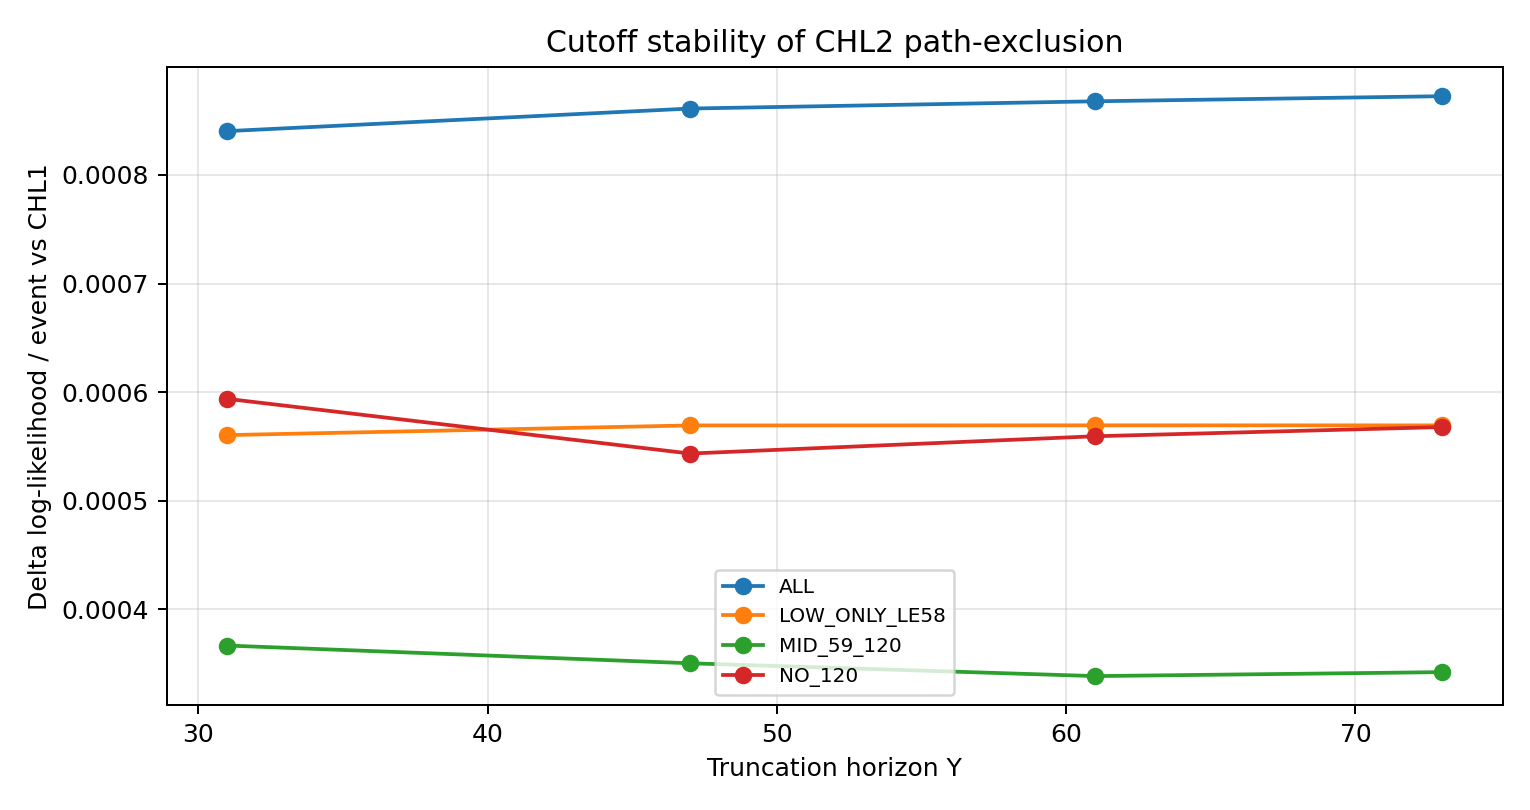
\includegraphics[width=0.88\textwidth]{figures/fig2_y_sweep_chl2_vs_chl1.png}\caption{Cutoff stability of CHL2 path-exclusion.}\end{figure}
\subsection{Stability against Cramer--Granville}
\begin{table}[H]\centering\small
\begin{tabular}{lrrr}
\toprule
Filter & min$_Y\Delta\ell$ vs CG gap-excl & mean$_Y\Delta\ell$ & positive $Y$ \\
\midrule
ALL & 0.422296 & 0.423471 & 4/4 \\
LOW\_ONLY\_LE58 & 0.330553 & 0.331239 & 4/4 \\
MID\_59\_120 & 2.411533 & 2.415574 & 4/4 \\
MID\_121\_240 & 5.034943 & 5.040513 & 4/4 \\
NO\_58 & 2.445323 & 2.449449 & 4/4 \\
NO\_120 & 5.039934 & 5.045511 & 4/4 \\
\bottomrule
\end{tabular}
\caption{Cutoff-stable CHL2 path-exclusion gain against the Cramer--Granville gap-exclusion order-zero baseline. These are conditional likelihood comparisons, not claims about extreme-gap asymptotics.}\label{tab:y-cg}\end{table}
These comparisons show that zero-memory spacing models do not capture the same conditional information as $P(g_2\mid g_1,x)$.
\begin{figure}[H]\centering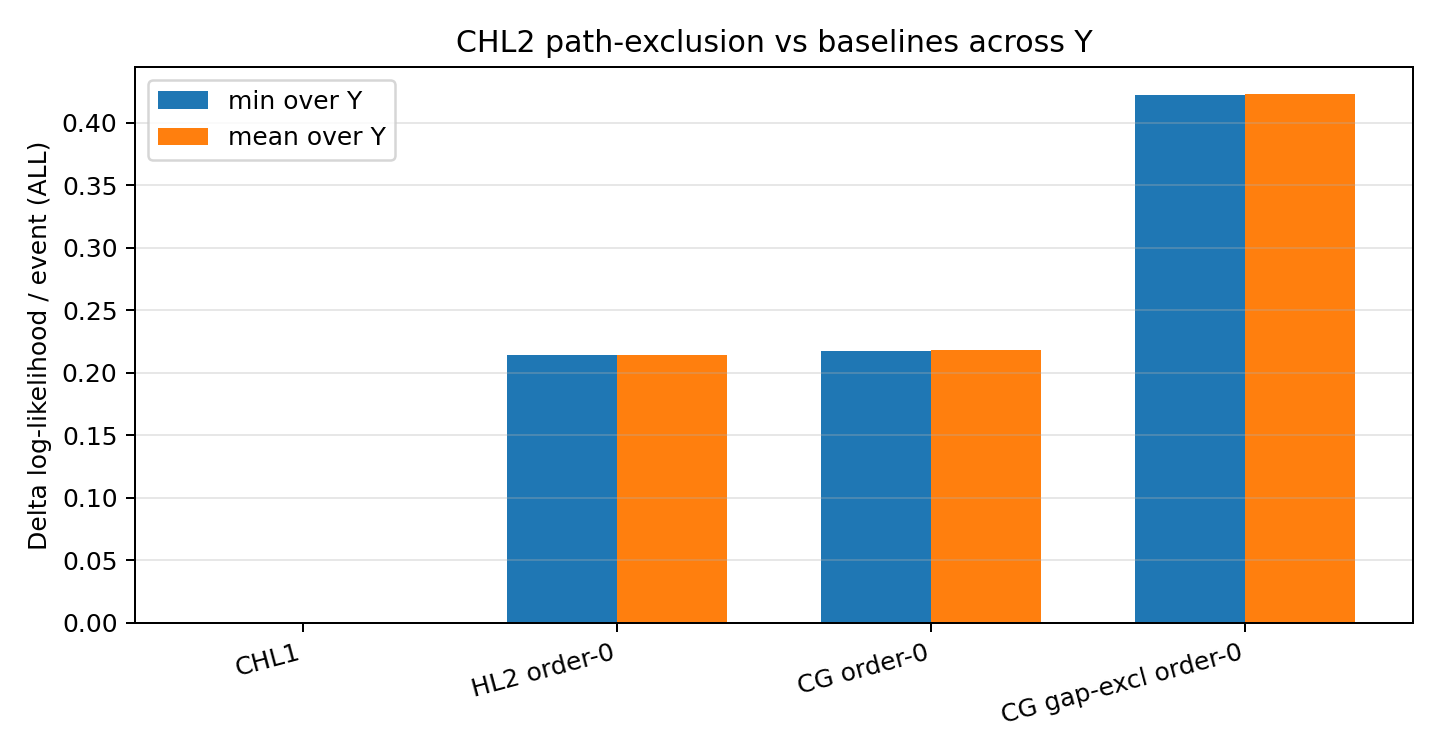
\includegraphics[width=0.88\textwidth]{figures/fig4_y_sweep_baselines_all.png}\caption{Full-support cutoff-stable gains of CHL2 path-exclusion against selected baselines.}\end{figure}
\subsection{Memory irreducibility}
\begin{table}[H]\centering\small
\begin{tabular}{lrrr}
\toprule
Filter & min$_Y\Delta\ell$ vs HL2 order-0 & min$_Y\Delta\ell$ vs CG order-0 & positive $Y$ \\
\midrule
ALL & 0.214011 & 0.217924 & 4/4 \\
MID\_59\_120 & 0.919981 & 1.280979 & 4/4 \\
MID\_121\_240 & 1.468296 & 2.576288 & 4/4 \\
NO\_58 & 0.977163 & 1.247847 & 4/4 \\
NO\_120 & 1.536290 & 2.572956 & 4/4 \\
\bottomrule
\end{tabular}
\caption{Operational irreducibility of the Markov memory. Entries are minimum gains over the tested $Y$ range.}\label{tab:memory}\end{table}
These are likelihood statements on the finite DS1 window: observing $g_1$ gives information about $g_2$ that is not recovered by the tested zero-memory models.

\section{Absolute prime-residue Oliver--Soundararajan diagnostic}
The final audit uses the chronological prime sequence and measures absolute prime-residue transitions $T_q^{\mathrm{emp}}(b,a)=P(p_i\equiv a\pmod q\mid p_{i-1}\equiv b\pmod q)$ for $q=3,5,7$. The theoretical matrix is generated from the CHL2 path kernel using the observed previous gap state, but not the target gap. Because the reduced space for $q=3$ has only two states, row-cosine alone is not used as an acceptance metric: row vectors close to the uniform vector can still produce cosines above $0.99$ even when the direction of the diagonal bias is wrong. For this reason the table reports the diagonal probability relative to the uniform diagonal baseline, and the qualitative sign of that diagonal displacement is treated as the decisive diagnostic for $q=3$.
\begin{table}[H]\centering\scriptsize
\resizebox{\textwidth}{!}{%
\begin{tabular}{lrrrrrrrll}
\toprule
$q$ & diagonal probability (empirical) & diagonal probability (CHL2) & uniform diagonal probability & row-cosine & KL & spectral-gap error & Pearson $\chi^2/N$ & diagonal sign & verdict \\
\midrule
3 & 0.455612 & 0.521890 & 0.500000 & 0.991261 & 0.008795 & 0.044996 & 0.017606 & empirical below / model above & wrong sign / limitation \\
5 & 0.192411 & 0.236270 & 0.250000 & 0.994572 & 0.005935 & 0.048890 & 0.011375 & both below & moderate \\
7 & 0.111342 & 0.130987 & 0.166667 & 0.998354 & 0.002076 & 0.019590 & 0.003996 & both below & strong \\
\bottomrule
\end{tabular}}
\caption{Absolute prime-residue diagnostic for CHL2 path-exclusion. The diagonal columns report $P(a=b)$ in the reduced residue transition matrix. Pearson $\chi^2/N$ is computed from empirical cell counts and CHL2 row probabilities. The row-cosine is included for comparability across moduli, but it is misleadingly optimistic in the two-state case $q=3$; the wrong-sign diagonal displacement and the largest $\chi^2/N$ value are the diagnostics that invalidate that case.}\label{tab:os}\end{table}
\subsection{$q=3$: wrong-sign low-modulus limitation}
Although the row-cosine is high in modulus $3$, the two-state nature of the reduced residue space makes that metric visually forgiving: vectors close to the uniform distribution are nearly collinear, so cosine values above $0.99$ are compatible with a wrong qualitative bias. The diagonal probability, or equivalently the sign of the diagonal displacement relative to the uniform value $1/2$, reveals the inversion. Empirically, the transition changes reduced class more often than it repeats it, with diagonal probability about $0.4556$, below the uniform value $0.5$. CHL2 predicts diagonal probability about $0.5219$, above uniform. The Pearson $\chi^2/N$ value is also largest for $q=3$ among the tested moduli. In a chi-square or signed-diagonal reading, this is not a marginal imperfection but a qualitative failure of the low-modulus prediction.

For a rigorous statistical treatment using the Pearson $\chi^2$ test, a dissection of the row-cosine metric illusion in binary systems, and the physical breakdown of the first-order Poisson survival approximation under high geometric compression, the reader is referred to Appendix~A.
\begin{table}[H]\centering\small
\begin{tabular}{llrr}
\toprule
from $b$ & to $a$ & empirical prob. & CHL2 prob. \\
\midrule
1 & 1 & 0.455636 & 0.522303 \\
1 & 2 & 0.544364 & 0.477697 \\
2 & 1 & 0.544413 & 0.478523 \\
2 & 2 & 0.455587 & 0.521477 \\
\bottomrule
\end{tabular}
\caption{Reduced prime-residue transition matrix for $q=3$. CHL2 predicts too much diagonal persistence, giving a qualitative wrong-sign result. The high row-cosine in Table~\ref{tab:os} should therefore not be interpreted as validation in this binary reduced space.}\label{tab:q3matrix}\end{table}
We treat this as a prominent limitation. It suggests that the first-order Poisson exclusion approximation is too coarse in the highly compressed low-wheel regime.
\subsection{$q=5$ and $q=7$: partial validation}
For $q=5$, CHL2 captures the direction of repulsion but softens its intensity: empirical diagonal probability is about $0.1924$, model diagonal probability about $0.2363$, and uniform reduced value $0.25$. For $q=7$, the fit is stronger: empirical diagonal probability is about $0.1113$, CHL2 about $0.1310$, and uniform reduced value $1/6\approx0.1667$. The row-cosine is $0.998354$ and the spectral-gap error is $0.019590$.
\begin{figure}[H]\centering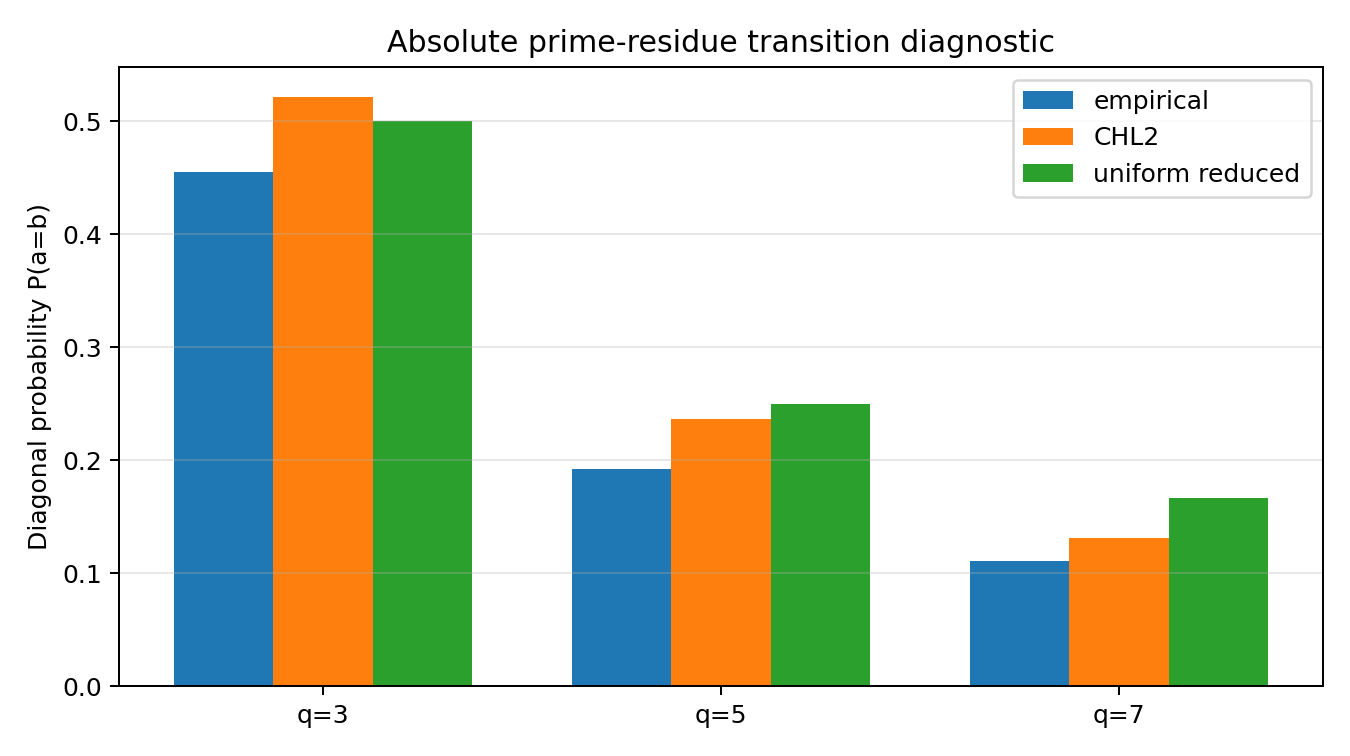
\includegraphics[width=0.78\textwidth]{figures/fig3_os_diagonal_probabilities.png}\caption{Absolute prime-residue transition diagnostic. CHL2 captures repulsion in $q=5,7$ but fails in $q=3$.}\end{figure}

\section{Limitations and falsification criteria}
\begin{enumerate}
\item \textbf{Wrong-sign modulus $3$ diagnostic.} CHL2 fails qualitatively in the two-state reduced residue transition for $q=3$. This is the most important modular limitation and should not be softened into a positive result. The failure is not fatal to the finite-window conditional gap likelihood results or to the behavior in higher reduced residue spaces, but it shows that the present CHL2 kernel is structurally insufficient for binary micro-biases on the lowest wheel.

\item \textbf{Low-wheel failure hypothesis.} Our working interpretation is that the $q=3$ anomaly exposes the theoretical limit of the first-order Poisson no-interior approximation in a regime of maximal geometric compression. In such a two-state reduced space, the potential interior-prime candidates are not weakly coupled: cross-dependencies between interior exclusions are strongest, and a product-style survival factor $\exp(-\Omegapath)$ can over-smooth the true class-switching bias. Capturing this regime would likely require second-order cluster or inclusion--exclusion terms coupling pairs of interior candidates. These terms are deliberately omitted in CHL2 to keep the kernel parameter-free and computationally auditable.

\item \textbf{First-order Poisson exclusion.} The no-interior factor $\Epath=\exp(-\Omegapath)$ omits second-order inclusion--exclusion or cluster corrections among multiple interior candidates. This is a controlled first-order approximation, not a final analytic expansion. The positive CHL2-vs-CHL1 gain validates this approximation only as a useful predictive correction, not as a derivation of exact independence among interior prime events.
\item \textbf{Local constant $\log x$.} The implementation uses a local constant $\log x$ in the interior intensity. This is appropriate for the narrow DS1 window but should be replaced by pointwise $\log(p_n+g_1+u)$ in scale-transfer audits.
\item \textbf{Finite truncation range.} The strongest cutoff sweep covers $Y=31,47,61,73$. It does not prove convergence as $Y\to\infty$.
\item \textbf{Single main scale.} The main DS1 window is near $10^{11}$. Transfer to other scales must be tested before any stronger universality claim.
\item \textbf{Sparse tails.} The \texttt{NO\_240} stratum has very low mass and should not be used as a central claim.
\end{enumerate}
The CHL2 interpretation would be weakened if the sign of the CHL2-vs-CHL1 gain became negative under a wider $Y$ sweep, if path-sensitive exclusion lost systematically to gap-only exclusion, if a new scale broke the same frozen formula, or if zero-memory Cramer--Granville baselines matched CHL2 under the same conditional protocol.
\section{Conclusion}
The CHL2 audit closes the current empirical phase with a cleaner object than the exploratory geometric models that preceded it. The kernel is built from two arithmetic operations: conditionalization of the Hardy--Littlewood singular series and a path-sensitive no-interior-prime survival factor. Both are parameter-free once the truncation horizon $Y$ and scale $x$ are fixed.

The empirical conclusions are stable and bounded. In DS1, CHL2 path-exclusion improves CHL1 ratio-only in every evaluated stratum. The improvement remains positive across $Y=31,47,61,73$. The model outperforms zero-memory baselines, including Cramer--Granville variants, in conditional likelihood. The absolute prime-residue diagnostic gives strong agreement in modulus $7$, moderate agreement in modulus $5$, and a wrong-sign limitation in modulus $3$ that identifies a real boundary of the present first-order approximation rather than a positive validation.
\[
\boxed{\text{Consecutive prime gaps admit a useful finite Markov factorization of Hardy--Littlewood structure.}}
\]
More precisely, the static triple-constellation weight becomes a conditional transition ratio, and the missing consecutiveness condition is approximated by a singular-series-weighted no-interior survival factor.
\section{Forward-looking remarks}
This final section is explicitly forward-looking. It is included to define possible next research directions and to prevent the empirical contribution from being confused with an announced proof. The proposals below are heuristic or programmatic unless explicitly stated otherwise; they are not part of the empirical validation claim of the paper.
\subsection{From conditional kernels to adaptive sieve weights}
CHL2 does not compete with classical sieves. It supplies a conditional target distribution that classical sieve weights do not usually define. A future adaptive sieve program could ask whether Selberg-type weights can be projected toward $P_{\CHLtwo}(h\mid g_1,x)$.

Let $w_\lambda(h)=\sum_{d\mid P_Y,\ d\mid h}\mu(d)\lambda_d$. A probabilistic reinterpretation of the squared weight gives
\[
P_{\mathrm{sieve},\lambda}(h\mid g_1,x)=\frac{w_\lambda(h)^2\oneadm(h;Y)}{\sum_k w_\lambda(k)^2\oneadm(k;Y)}.
\]
The direct information-theoretic projection is the heuristic objective
\[
J(\lambda)=D_{\mathrm{KL}}\!\left(P_{\mathrm{sieve},\lambda}(\cdot\mid g_1,x)\ \|\ P_{\CHLtwo}(\cdot\mid g_1,x)\right)+\kappa\sum_{d\mid P_Y}\frac{\lambda_d^2}{d}.
\]
This is a heuristic proposal and not a proven result. Sieve weights are not normally probability measures over gaps, and the entropy of $P_{\mathrm{sieve},\lambda}$ is not constant because it depends on $\lambda$.

A first-order linearization suggests the working form
\[
\lambda_d^\star \propto \mu(d)\cdot \mathbb{E}_{h\sim\mathrm{adm}}\!\left[\log\frac{1}{P_{\CHLtwo}(h\mid g_1,x)}\ \middle|\ d\mid h\right],
\]
possibly with centering by the unconditional admissible average. This expression is a conjectural linearization, not a theorem; a full variational analysis would require controlling the dependence of the sieve-induced distribution on $\lambda$. The conceptual point is that optimal coefficients would no longer depend only on a homogeneous cutoff such as $\log(R/d)$; they would depend on the local CHL2 conditional log-potential.

This connects naturally with local-level and weighted-sieve literature, including Barban--Vehov/Selberg mean-square themes, the Barban--Davenport--Halberstam tradition, and the Friedlander--Iwaniec framework \cite{barban1961,barban-vehov,bfi1986,friedlander-iwaniec}. The proposed novelty is not the existence of weights, but the explicit path-dependent target distribution.
\subsection{Connection with Maynard--Tao weights}
Maynard--Tao weights are designed to detect multiple primes inside translated admissible tuples. A CHL2-guided variant would not replace that functional. It would reinterpret small configurations, especially $k=2$ or $k=3$, as conditional transitions. For example, a twin-prime channel could be studied as a transition involving $g_1=2$ and a candidate next gap $g_2$, weighted by the conditional singular-series ratio and the no-interior survival factor.

This is proposed as an outlook, not as an announced improvement to Maynard--Tao theorems. The analytic obstacles are significant: conditioning on a previous gap changes the averaging structure and can interfere with the factorization properties that make standard sieve estimates tractable.
\subsection{Computational outlook: prioritized search and Hit@K}
The CHL2 cost $\mathcal C_Y(g_2\mid g_1;x)=-\log R_Y(g_2\mid g_1)+\Omegapath(g_1,g_2;x)$ can be used as a parameter-free ranking oracle for candidate continuations of a prime-gap path. A natural benchmark is Hit@K: among the top $K$ candidate gaps ranked by $\mathcal C_Y$, how often does the true next gap appear? Such a benchmark would not prove a theorem, but it could establish practical value in search prioritization for rare constellations, structured prime patterns, or candidate record gaps.
\appendix
\renewcommand{\thesection}{Appendix \Alph{section}:}
\section{The $q=3$ Anomaly and Limits of the First-Order Poisson Approximation}\label{app:q3}

This appendix isolates a small but important failure mode of the CHL2 kernel.  The main likelihood audits show that the path-sensitive no-interior correction improves the conditional Hardy--Littlewood Markov kernel over CHL1 and over zero-memory baselines.  However, the absolute prime-residue Oliver--Soundararajan diagnostic reveals that the reduced residue system modulo $3$ is not correctly reproduced by the present first-order model.

\subsection*{A.1. Why row-cosine is insufficient in a two-state reduced residue space}

For a modulus $q$, let
\[
T_q^{\mathrm{emp}}(b,a)=\mathbb{P}_{\mathrm{emp}}(p_i\equiv a\pmod q\mid p_{i-1}\equiv b\pmod q)
\]
be the empirical transition matrix on reduced prime residues, and let $T_q^{\mathrm{CHL2}}(b,a)$ be the matrix induced by the CHL2 path-exclusion kernel.  In the reduced system modulo $3$, the state space contains only two classes, $\{1,2\}$.  In such a two-state space, row-cosine similarity is a visually forgiving metric: two probability vectors close to $(1/2,1/2)$ can have cosine similarity exceeding $0.99$ even when the diagonal/off-diagonal bias has the wrong sign.

For this reason, the diagnostic table reports not only row-cosine and KL divergence, but also the diagonal probability and a Pearson chi-square statistic.  The diagonal probability is
\[
D_q(T)=\sum_b \pi_b T_q(b,b),
\]
where $\pi_b$ is the empirical row mass.  In the OS run, the empirical and CHL2 diagonal masses were
\[
D_3(T^{\mathrm{emp}})=0.455612,
\qquad
D_3(T^{\mathrm{CHL2}})=0.521890,
\qquad
D_3(T^{\mathrm{uniform}})=0.500000.
\]
Thus the empirical transition prefers changing reduced residue class modulo $3$, whereas CHL2 predicts excess persistence.  This is a qualitative wrong-sign failure.  The high row-cosine value in this case must therefore not be interpreted as a successful reproduction of the modulo-$3$ transition bias.

\subsection*{A.2. Pearson chi-square diagnostic}

Let $O_{ba}$ denote the observed transition count from $b$ to $a$, and let
\[
E_{ba}=N_b\,T_q^{\mathrm{CHL2}}(b,a),
\qquad
N_b=\sum_a O_{ba},
\]
be the expected count under the CHL2 transition matrix, row-normalized to the empirical number of transitions leaving $b$.  The Pearson statistic is
\[
\chi_q^2=\sum_{b}\sum_{a}\frac{(O_{ba}-E_{ba})^2}{E_{ba}},
\]
with rows restricted to positive empirical mass.  For rows with $m_q$ positive expected cells, the nominal degrees of freedom are summed as
\[
\mathrm{df}_q=\sum_{b:N_b>0}(m_q(b)-1).
\]
The normalized statistic $\chi_q^2/N$ is especially useful for comparing moduli with different state-space sizes.

For the absolute prime-residue OS diagnostic on DS1, the Pearson summaries were:
\[
\begin{array}{c|r|r|r|r|r|r}
q & N & \chi^2 & \mathrm{df} & \chi^2/N & D_q(T^{\mathrm{emp}}) & D_q(T^{\mathrm{CHL2}})\\
\hline
3 & 78{,}934{,}823 & 1{,}389{,}703.35 & 2 & 0.017606 & 0.455612 & 0.521890\\
5 & 78{,}934{,}823 & 897{,}882.34 & 12 & 0.011375 & 0.192411 & 0.236270\\
7 & 78{,}934{,}823 & 315{,}442.52 & 30 & 0.003996 & 0.111342 & 0.130987
\end{array}
\]
The modulo-$7$ case is the strongest agreement: both empirical and modeled diagonal probabilities lie below the uniform diagonal probability $1/6$, and the chi-square per transition is smallest.  Modulo $5$ is intermediate: CHL2 captures the direction of repulsion but smooths its intensity.  Modulo $3$ fails qualitatively because the diagonal bias crosses the uniform baseline in the wrong direction.

\subsection*{A.3. Interpretation: compression of the reduced wheel modulo $3$}

We interpret the modulo-$3$ anomaly as a limit of the first-order Poisson no-interior-prime approximation in a maximally compressed reduced residue system.  The CHL2 path-exclusion factor is
\[
E_Y^{\mathrm{path}}(g_1,g_2;x)=\exp\{-\Omega_Y^{\mathrm{path}}(g_1,g_2;x)\},
\]
where
\[
\Omega_Y^{\mathrm{path}}(g_1,g_2;x)=\sum_{\substack{2\le u\le g_2-2\\ u\ \mathrm{even}}}\frac{\mathfrak S_Y(\{0,g_1,g_1+u,g_1+g_2\})}{\mathfrak S_Y(\{0,g_1,g_1+g_2\})}\frac{1}{\log x}.
\]
This is a first-order survival approximation: it sums the conditional Hardy--Littlewood intensity of possible interior primes and exponentiates the negative expected count.  In doing so, it treats the interior-prime events as weakly dependent.  That approximation is adequate as a parameter-free correction for the main conditional gap likelihood, but it is not designed to capture the strongest micro-scale modular repulsion in a two-state reduced space.

Modulo $3$, the reduced residue space has only two viable states.  The local geometry is therefore highly compressed: any excess persistence or excess switching immediately dominates the entire transition matrix.  In this regime, the dependence between possible interior-prime candidates is strongest.  If one interior candidate is excluded, the conditional probability of the next nearby candidate is not merely adjusted by an independent Poisson survival factor; it is altered by local inclusion-exclusion structure among pairs of interior candidates.

A second-order cluster correction would introduce terms of the schematic form
\[
\Omega_Y^{(2)}=\Omega_Y^{(1)}-\frac12\sum_{u\ne v}\Delta_Y(u,v\mid H_3)+\cdots,
\]
where
\[
\Delta_Y(u,v\mid H_3)=\frac{\mathfrak S_Y(H_5(u,v))}{\mathfrak S_Y(H_3)}-\frac{\mathfrak S_Y(H_4(u))}{\mathfrak S_Y(H_3)}\frac{\mathfrak S_Y(H_4(v))}{\mathfrak S_Y(H_3)},
\]
with
\[
H_3=\{0,g_1,g_1+g_2\},\quad
H_4(u)=\{0,g_1,g_1+u,g_1+g_2\},
\]
and
\[
H_5(u,v)=\{0,g_1,g_1+u,g_1+v,g_1+g_2\}.
\]
Such terms are omitted deliberately in CHL2.  The present model keeps only the first-order Poisson survival factor in order to remain parameter-free, computationally feasible, and directly interpretable.  The modulo-$3$ failure therefore marks a boundary of the approximation, not a hidden success.

\subsection*{A.4. Consequence for the claims of the paper}

The $q=3$ anomaly is not fatal to the main CHL2 claim.  The main claim concerns conditional gap prediction and the path-sensitive improvement of CHL2 over CHL1 and zero-memory baselines.  Those likelihood gains are stable across filters, blocks, and the evaluated truncation horizons.  The anomaly does, however, show that CHL2 in its present form is structurally insufficient for micro-biases in binary reduced residue systems.  Consequently, the paper treats modulo $3$ as a failure mode of the first-order model and not as positive validation.

This distinction is essential.  CHL2 is a strong first-order conditional kernel for consecutive prime gaps; it is not a complete model of every low-modulus residue bias.  A future CHL3-style refinement would need to test whether second-order inclusion-exclusion or cluster corrections repair the $q=3$ wrong-sign effect without degrading the parameter-free likelihood gains that make CHL2 useful.

\section{Reproducibility summary}
The CHL2 audits used ten parent-wide DS1 blocks and the real chronological prime sequence for the absolute residue diagnostic. The main run used $Y=47$ as truncation horizon, path-exclusion enabled, and all blocks B01--B10. The cutoff sweep used $Y\in\{31,47,61,73\}$. The OS absolute run used $q=3,5,7$ and the model \texttt{CHL2\_path\_excl\_cond\_eta}. The path-exclusion cache is an acceleration artifact and not a fitted model object.
\section{AI-assisted workflow disclosure}
The author used AI-assisted systems, including ChatGPT, Gemini, and related tools, as interactive research assistants during exploratory, coding, diagnostic, and drafting phases. Their use included code prototyping, debugging, construction of diagnostic tests, adversarial critique of hypotheses, summarization of numerical outputs, and drafting support. All experiments were executed locally by the author. All reported claims, mathematical formulations, code selections, and interpretations were reviewed and curated by the author, who assumes full responsibility for the manuscript. No AI system is listed as an author.
\begin{thebibliography}{99}
\bibitem{barban1961} M. B. Barban, \emph{New applications of the large sieve of Yu. V. Linnik}, Trudy Inst. Mat. Akad. Nauk UzSSR \textbf{22} (1961), 1--20.
\bibitem{barban-vehov} V. K. Murty, \emph{The Barban--Vehov theorem in arithmetic progressions}, Hardy-Ramanujan Journal \textbf{41} (2018), 157--171.
\bibitem{bfi1986} E. Bombieri, J. B. Friedlander, and H. Iwaniec, \emph{Primes in arithmetic progressions to large moduli}, Acta Mathematica \textbf{156} (1986), 203--251.
\bibitem{cramer1936} H. Cramer, \emph{On the order of magnitude of the difference between consecutive prime numbers}, Acta Arithmetica \textbf{2} (1936), 23--46.
\bibitem{ford2016} K. Ford, B. Green, S. Konyagin, J. Maynard, and T. Tao, \emph{Long gaps between primes}, Journal of the American Mathematical Society \textbf{31} (2018), 65--105.
\bibitem{friedlander-iwaniec} J. Friedlander and H. Iwaniec, \emph{Opera de Cribro}, American Mathematical Society Colloquium Publications, Vol. 57, American Mathematical Society, 2010.
\bibitem{gpy} D. A. Goldston, J. Pintz, and C. Y. Yildirim, \emph{Primes in tuples I}, Annals of Mathematics \textbf{170} (2009), 819--862.
\bibitem{granville1995} A. Granville, \emph{Harald Cramer and the distribution of prime numbers}, Scandinavian Actuarial Journal \textbf{1995} (1995), 12--28.
\bibitem{hardy-littlewood} G. H. Hardy and J. E. Littlewood, \emph{Some problems of Partitio Numerorum III: On the expression of a number as a sum of primes}, Acta Mathematica \textbf{44} (1923), 1--70.
\bibitem{lemke-sound} R. J. Lemke Oliver and K. Soundararajan, \emph{Unexpected biases in the distribution of consecutive primes}, Proceedings of the National Academy of Sciences \textbf{113} (2016), E4446--E4454.
\bibitem{maynard-large} J. Maynard, \emph{Large gaps between primes}, Annals of Mathematics \textbf{183} (2016), 915--933.
\bibitem{maynard-small} J. Maynard, \emph{Small gaps between primes}, Annals of Mathematics \textbf{181} (2015), 383--413.
\bibitem{selberg} A. Selberg, \emph{On elementary methods in prime number theory and their limitations}, in \emph{Collected Papers}, Vol. I, Springer, 1989.
\bibitem{zhang} Y. Zhang, \emph{Bounded gaps between primes}, Annals of Mathematics \textbf{179} (2014), 1121--1174.
\end{thebibliography}
\end{document}
